\chapter{RELATED THEORY}

\section{Monolithic Architecture}
A monolithic architecture is a software design pattern where all components of an application are integrated into a single code base. This approach simplifies deployment and management, as all functionalities are contained within a single codebase. It can be faster in handling requests when the number of requests is fixed and the load is less \cite{8928192}.

\section{MVVM Architecture}
Model-View-ViewModel (MVVM) is a software architectural pattern that facilitates the separation of the development of the graphical user interface (the view) from the development of the business logic or back-end logic (the model). The view model of MVVM is a value converter, meaning the view model is responsible for exposing (converting) the data objects from the model in such a way that objects are easily managed and presented. This pattern is particularly useful in mobile application development for maintaining a clean separation of concerns and enhancing testability \cite{fowler2025presentationmodel}.

\begin{figure}[H]
    \centering
    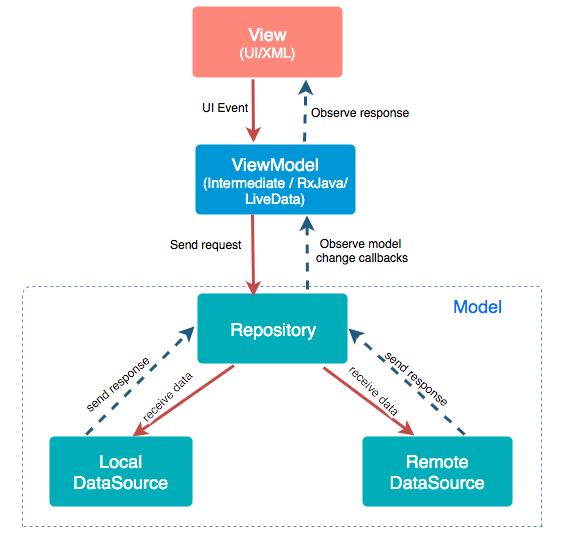
\includegraphics[width=0.8\textwidth]{Graphics/mvvm_architecture.png}
    \caption{MVVM Architecture}
    \label{fig:mvvm_architecture}
\end{figure}

\section{REST API}
REST (Representational State Transfer) is an architectural approach for developing web services. A RESTful API (Application Programming Interface) is built using REST concepts. RESTful APIs transfer a representational state of the resource to the endpoint or requester. The information can be of any format like JSON, HTML, PHP, XML, etc.

REST APIs are used for data exchange between client and server. They communicate with the server via HTTP (Hypertext Transfer Protocol) techniques. The most often used HTTP methods in RESTful APIs are GET, POST, PUT, PATCH, and DELETE.

\subsection{GET}
The GET method is used when data is needed to retrieve from the server. It reads the data from the server. It is used to retrieve data like user profiles, product information, or other resources.

\subsection{POST}
The POST method is used to send data to the server. It is useful for creating new resources to be retrieved later on the server.

\subsection{PUT}
The PUT method is used to update an existing resource on the server. It replaces the existing resource with the new one that is sent in the request.

\subsection{PATCH}
The PATCH method is similar to the PUT method, but it only updates the specified fields of an existing resource. It is used when only a portion of a resource needs to be updated, rather than replacing the entire resource.

\subsection{DELETE}
The DELETE method is used to delete a resource from the server. It removes the resource from the server and makes it unavailable for further use.